\def\sode{8}
\begin{name}
	{\tenchude}
	{\tendethi}
	{\tentruong}
	{\thoigian}
\end{name}
\caulc
\Opensolutionfile{ans}[ans/ans-HXN-\sode-T]
\begin{ex}%Câu 1
\immini
{
     Hình vẽ bên là đồ thị của hàm số $y=\dfrac{ax+b}{cx+d}$ . Đường tiệm cận đứng của đồ thị hàm số có phương trình là 
 \choice
 {\True $x=1$}
 {$x=2$}
 {$y=1$}
 {$y=2$}
}
{
    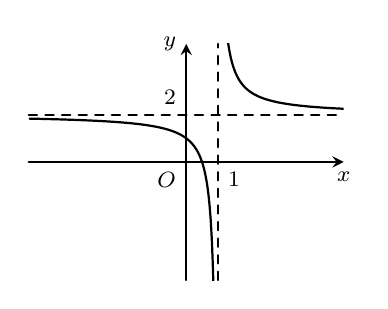
\begin{tikzpicture}[>=stealth, line join=round, line cap=round, font=\footnotesize, scale=1, declare function={a=2; b=-1; c=1; d=-1; hsf(\x)=(a*\x+b)/(c*\x+d);},x=.4cm,y=.3cm,thick]
        \draw[->] (-5,0) -- (5,0)node[below]{$x$};
        \draw[->] (0,-5) -- (0,5)node[left]{$y$};
        \draw (0,0) node[below left]{$O$}
        (1,0)node[below right]{$1$}
        (0,2)node[above left]{$2$};
        \draw[dashed] ({-d/c},-5)--({-d/c},5) (-5,{a/c})--(5,{a/c});
        \clip (-5,-5) rectangle (5,5);
        \pgfmathsetmacro{\can}{-d/c}
        \draw[,samples=150,smooth,domain=-5:{\can-.1}] plot(\x,{hsf(\x)});
        \draw[,samples=150,smooth,domain={\can+.1}:5] plot(\x,{hsf(\x)});
    \end{tikzpicture}
}
\end{ex}
\begin{ex}%Câu 2
 Gọi $S$ là diện tích của hình phẳng giới hạn bởi các đường $y=5^x$, $y=0$, $x=0$, $x=2$. Mệnh đề nào dưới đây đúng?
 \choice
 {\True $S=\int\limits_0^25^x\text{d}x$}
 {$S=\pi\int\limits_0^25^{2x}\text{d}x$}
 {$S=\dfrac{1}{\ln 5}\int\limits_0^25^x\text{d}x$}
 {$S=\ln 5\int\limits_0^25^x\text{d}x$}
\end{ex}
\begin{ex}%Câu 3
 Giá trị lớn nhất của hàm số $f(x)=x^3-3x^2-9x+10$ trên đoạn $\left[-2;2\right]$ bằng
 \choice
 {$-12$}
 {$10$}
 {\True $15$}
 {$-2$}
\end{ex}
\begin{ex}%Câu 4
 Cho hàm số $y=f(x)$ có bảng xét dấu đạo hàm như sau:\\
 \centerline{
 
\begin{tikzpicture}
     \tkzTabInit[nocadre=false,lgt=1.4,espcl=3,deltacl=0.5]{$x$/.7,$f'(x)$/.7}
     {$-\infty$ , $-1$ , $0$ , $1$ , $+\infty$}
     \tkzTabLine{, - , $0$ , + , $0$ , - , $0$ , + }
 \end{tikzpicture}
 }
 Hàm số$f(x)$ đồng biến trên khoảng nào sau đây?
 \choice
 {$\left(0;1\right)$}
 {$\left(-1;0\right)$}
 {\True $\left(-\infty;-1\right)$}
 {$\left(-1;+\infty\right)$}
\end{ex}
\begin{ex}%Câu 5
 Tập nghiệm của bất phương trình $3^{2x-1}>27$ là
 \choice
 {$\left(\dfrac{1}{2};+\infty\right)$}
 {$\left(3;+\infty\right)$}
 {\True $\left(2;+\infty\right)$}
 {$\left(\dfrac{1}{3};+\infty\right)$}
\end{ex}
\begin{ex}%Câu 6
 Tìm nguyên hàm $F(x)$ của hàm số $f(x)=\sin x+\cos x$ thoả mãn $F\left(\dfrac{\pi}{2}\right)=2$.
 \choice
 {$F(x)=-\cos x+\sin x+3$}
 {$F(x)=-\cos x+\sin x-1$}
 {\True $F(x)=-\cos x+\sin x+1$}
 {$F(x)=\cos x-\sin x+3$}
\end{ex}
\begin{ex}%Câu 7
 Cho cấp số cộng $\left(u_n\right)$ với năm số hạng đầu là $2$; $7$; $12$; $17$; $22$. Số hạng tổng quát của cấp số cộng là
 \choice
 {$u_n=3n+5$}
 {$u_n=3n-5$}
 {$u_n=5n+3$}
 {\True $u_n=5n-3$}
\end{ex}
\begin{ex}%Câu 8
 Bảng dưới đây thống kê cự li ném tạ trong quá trình luyện tập của một vận động viên trong một tuần (đơn vị: mét).\\
 \centerline{\begin{tabular}{|c|c|c|c|c|c|}
 \hline
 Cự li (m) & $\left[19;19,5\right)$ & $\left[19,5;20\right)$ & $\left[20;20,5\right)$ & $\left[20,5;21\right)$ & $\left[21;21,5\right)$\\
 \hline
 Tần số & 13 & 45 & 24 & 12 & 6\\
 \hline
 \end{tabular}}\\
 Hãy tính phương sai của mẫu số liệu ghép nhóm trên (làm tròn đến hàng phần nghìn).
 \choice
 {\True $0{,}277$}
 {$0{,}526$}
 {$0{,}326$}
 {$0{,}211$}
 \end{ex}
\begin{ex}%Câu 9
 Cho hai mặt phẳng $(P)\colon 2x-y-z-3=0$ và $(Q)\colon x-z-2=0$. Góc giữa hai mặt phẳng $(P)$ và $(Q)$ bằng
 \choice
 {\True $30^{\circ}$}
 {$45^{\circ}$}
 {$60^{\circ}$}
 {$90^{\circ}$}
\end{ex}
\begin{ex}%Câu 10
 Khảo sát thời gian tập thể dục của một số học sinh khối 11 thu được mẫu số liệu ghép nhóm sau:\\
\centerline{
\begin{tblr}{colspec={|c|c|c|c|c|c|}, hlines, vlines}
    Thời gian (phút) & [0;20) & [20;40) & [40;60) & [60;80) & [80;100) \\
    Số học sinh & 5 & 9 & 12 & 10 & 6 \\
\end{tblr}
}
 Mốt của mẫu số liệu ghép nhóm trên là
 \choice
 {\True $52$}
 {$42$}
 {$53$}
 {$54$}
\end{ex}
\begin{ex}%Câu 11
 Một vật chuyển động có phương trình $s(t)=3\cos t$ . Khi đó, vận tốc tức thời tại thời điểm $t$ của vật là:
 \choice
 {\True $v(t)=-3\sin t$}
 {$v(t)=-3\cos t$}
 {$v(t)=3\cos t$}
 {$v(t)=3\sin t$}
\end{ex}
\begin{ex}%Câu 12
 Trong không gian $Oxyz$ , một vectơ pháp tuyến của mặt phẳng $\dfrac{x}{-2}+\dfrac{y}{-1}+\dfrac{z}{3}=1$ là
 \choice
 {\True $\vec{n}=(3;6;-2)$}
 {$\vec{n}=(2;-1;3)$}
 {$\vec{n}=(-3;-6;-2)$}
 {$\overrightarrow{n}=(-2;-1;3)$}
 \end{ex}
\Closesolutionfile{ans}
\cauds
\Opensolutionfile{ans}[ans/ans-HXN-\sode-TF]
\begin{ex}%Câu 13
 Cho hàm số $y=f(x)=\dfrac{x-m^2+m}{x+1}$ , $m$ là tham số.
 \choiceTF
 {Với $m=1$ thì hàm số $y=f(x)$ luôn nghịch biến trên các khoảng $\left(-\infty;-1\right)$ và $\left(-1;+\infty\right)$}
 {\True Với mọi số thực $m$ thì hàm số $y=f(x)$ luôn đồng biến trên các khoảng $\left(-\infty;-1\right)$ và $\left(-1;+\infty\right)$}
 {\True $\underset{\left[1;2\right]}{\max}f(x)=f(2)$}
 {\True Có hai giá trị nguyên $m$ để $\underset{\left[0;1\right]}{\min}f(x)=-2$}
\end{ex}
\begin{ex}%Câu 14
\immini
{
    Một vật chuyển động trong $3$ giờ với vận tốc $v$ (km/h) phụ thuộc vào thời gian $t$ (h), đồ thị của hàm vận tốc được cho như hình vẽ. Trong thời gian $1$ giờ kể từ khi vật bắt đầu chuyển động, đồ thị hàm vận tốc của nó là một phần của parabol có đỉnh $S(2;9)$ , khoảng thời gian còn lại đồ thị là một đoạn thẳng song song với trục hoành.
 \choiceTF
 {\True Tại thời điểm bắt đầu chuyển động, vật có vận tốc bằng $4$ km/h}
 {Trong thời gian $1$ giờ kể từ khi bắt đầu chuyển động, phương trình vận tốc của vật là $v(t)=-\dfrac{5}{4}{t^2}-5t+4$}
 {\True Sau $30$ phút kể từ khi bắt đầu chuyển động, gia tốc của vật bằng $3,75$ km/h$^2$}
 {\True Quãng đường $S$ mà vật đi được được trong $3$ giờ (làm tròn đến hàng phần trăm) là $21{,}58$ km}
}
{
    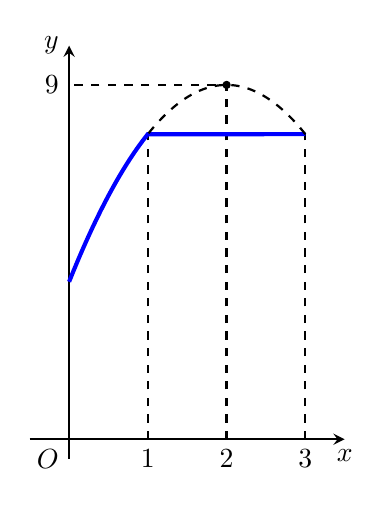
\begin{tikzpicture}[>=stealth, thick, scale=1, declare function={a=-5/4; b=5; c=4; hsf(\x)=a*(\x)^2+b*\x+c;},y=.5cm]
        \draw[->] (-.5,0) -- (3.5,0)node[below]{$x$};
        \draw[->] (0,-.5) -- (0,10)node[left]{$y$};
        \draw (0,0) node[below left]{$O$};
        \draw[dashed]  (2,0) node[below]{$2$} |-(0,9) node[left]{$9$}
        (1,0)node[below]{$1$}--(1,{hsf(1)})
        (3,0)node[below]{$3$}--(3,{hsf(3)});
        \fill (2,{hsf(2)}) circle (1.5pt);
        \draw[samples=150, smooth,line width=1.5pt,blue , domain=0:1] plot(\x,{hsf(\x)})--(3,{hsf(3)});
        \draw[samples=150, smooth, dashed, domain=3:1] plot(\x,{hsf(\x)});
    \end{tikzpicture}
}
\end{ex}
\begin{ex}%Câu 15
Trong một căn phòng có chiều ngang $4$ m, chiều rộng $8$ m và chiều cao $4$ m, người chủ đã thiết kế $4$ dãy đèn led chạy dọc theo các đường chéo của hình chữ nhật tương ứng với các bức tường căn phòng sao cho chúng có tính liên tục. Thiết lập hệ trục tọa độ Oxyz như hình vẽ với căn phòng là hình hộp chữ nhật $ABCD.A'B'C'D'$ , trong đó điểm $A$ là gốc tọa độ, đơn vị trên mỗi trục là mét.
\begin{center}
    \includegraphics[width=5cm]{img/HXN-8-15a}\qquad \includegraphics[width=5cm]{img/HXN-8-15b}
\end{center}
 Chủ căn phòng quyết định sử dụng loại đèn LED neon Flex (không chói mắt) với giá thị trường khoảng 85 nghìn đồng/mét.\\
 \choiceTF
 {Phương trình cạnh BD là $\heva{& x=0\\& y=4+t\\& z=t}$ ($t$ là tham số)}
 {\True Số tiền để mua đèn led trang trí trong căn phòng là $2482$ (nghìn đồng), làm tròn đến hàng đơn vị của nghìn đồng}
 {Khoảng cách từ $D$ đến mặt phẳng $\left(A'B'C'\right)$ bằng $5{,}2$m (làm tròn đến hàng phần chục)}
 {Biết đèn LED có điểm sáng $M$ chạy từ $B$ đến $D$ với tốc độ $0{,}2$ m/s , đèn LED có điểm sáng $N$ chạy từ $A'$ đến $C'$ với tốc độ $0{,}3$ m/s. Sau $9{,}1$ giây (làm tròn đến hàng phần chục) kể từ khi mở nguồn thì hai điểm sáng $M$, $N$ có khoảng cách ngắn nhất trước khi có ít nhất một điểm sáng về đích}
 \loigiai{
 \begin{itemchoice}
     \itemch 
     \itemch 
     \itemch 
     \itemch 
     Ta có $\vec{BD}=(0;-4;4)\Rightarrow \vec{u}=0{,}2\times \dfrac{1}{BD}\vec{BD}=\left(0;-\dfrac{\sqrt{2}}{10};\dfrac{\sqrt{2}}{10}\right)$ là vectơ chỉ phương của $BD$.\\
     Điểm $M\in BD$ nên tại thời điểm $t$, điểm $M$ ở vị trí $M\left( 0;4-\dfrac{\sqrt{2}}{10}t;\dfrac{\sqrt{2}}{10}t \right)$\\
     Ta có $\vec{A'C'}=(0;4;4)\Rightarrow \vec{v}=0{,}3\times \dfrac{1}{A'C'}\vec{A'C'}=\left(0;\dfrac{3\sqrt{2}}{20};\dfrac{3\sqrt{2}}{20}\right)$ là vectơ chỉ phương của $A'C'$.\\
     Điểm $N\in A'C'$ nên tại thời điểm $t$, điểm $N$ ở vị trí $N\left(8;\dfrac{3\sqrt{2}}{20}t;\dfrac{3\sqrt{2}}{20}t\right)$.\\
     Do đó $\vec{MN}=\left(8;\dfrac{\sqrt{2}}{4}t-4;\dfrac{\sqrt{2}}{20}t\right)$\\
     $\Rightarrow MN^2=8^2+\left(\dfrac{\sqrt{2}}{4}t-4\right)^2+\left(\dfrac{\sqrt{2}}{20}t\right)^2=\dfrac{13}{100}t^2-2\sqrt{2}t+80$.\\
     Dễ thấy $MN=\sqrt{\dfrac{13}{100}t^2-2\sqrt{2}t+80}$ đạt giá trị nhỏ nhất $MN_{\min }\approx 8{,}04$; khi đó $t\approx 10{,}9$  giây.
     \end{itemchoice}
 }
\end{ex}
\begin{ex}%Câu 16
Hộp I đựng $3$ bi xanh và $2$ bi vàng; hộp II có $3$ bi xanh, $1$ bi đen và $1$ bi vàng; hộp III có $1$ bi xanh, $1$ bi đen và $3$ bi vàng. Lấy ngẫu nhiên $1$ viên bi từ hộp I bỏ sang hộp II; đồng thời lấy ngẫu nhiên 1 viên bi từ hộp III bỏ sang hộp II; sau đó lấy ngẫu nhiên $2$ viên bi từ hộp II.\\
\centerline{
\includegraphics[width=6cm]{img/HXN-8-16}
}
 \choiceTF
 {Xác suất để hộp thứ II nhận được 2 bi cùng màu bằng $\dfrac{8}{25}$}
 {\True Xác suất để lấy được 2 bi đen từ hộp II bằng $\dfrac{1}{105}$}
 {\True Xác suất để lấy được 2 bi vàng từ hộp II bằng $\dfrac{31}{525}$}
 {Xác suất để lấy được 2 bi từ hộp II cũng là 2 bi được chuyển sang từ hai hộp I, III bằng $\dfrac{5}{31}$ , biết rằng đó là 2 viên bi vàng}
\end{ex}
\Closesolutionfile{ans}
\caukq
\Opensolutionfile{ans}[ans/ans-HXN-\sode-SA]
\begin{ex}%Câu 17
 \immini
 {
     Một người đưa thư xuất phát từ bưu điện (vị trí A) và phải đi qua các con đường để phát thư trước khi quay trở lại bưu điện. Sơ đồ các con đường cần đi qua và độ dài của chúng (tính theo mét) được biểu diễn ở hình vẽ dưới. Hỏi người đó phải đi như thế nào để đường đi là ngắn nhất?
 \shortans{8300}
 }
 {
     \includegraphics[width=6cm]{img/HXN-8-17}
 }
 \end{ex}
 \begin{ex}%Câu 18
Cho đồ thị hàm số $y=\sqrt{x^2-4x+3}$ có các đường tiệm cận xiên $d_1$ và $d_2$ . Tìm tổng khoảng cách từ gốc tọa độ đến hai đường tiệm cận xiên $d_1,d_2$ (kết quả được làm tròn đến hàng phần trăm).
\shortans{2,83}
\end{ex}
\begin{ex}%Câu 19
\immini
{
    Một chiếc bánh kem mừng sinh nhật có dạng hình chóp cụt đều $ABC.A'{B}'{C}'$ với cạnh đáy lớn bằng $4$dm, cạnh đáy nhỏ bằng $2$dm và chiều cao của nó bằng $1{,}5$dm . Tìm thể tích của chiếc bánh kem đó theo đơn vị $d$ m$^3$ (làm tròn đến hàng phần trăm, bỏ qua những thứ trang trí quanh chiếc bánh).
\shortans{6,06}
}
{
    \includegraphics[width=6cm]{img/HXN-8-19-LG}
}
\loigiai{
\immini
{
    Xét hình chóp cụt đều $ABC.A'B'C'$ như hình vẽ; trong đó chiều cao $h=IO=1{,}5$dm.\\
Diện tích hai đáy hình chóp cụt đều $S_1=S_{\triangle ABC}=\dfrac{4^2\sqrt{3}}{4}=4\sqrt{3}\,dm^2$; $S_2=S_{\triangle A'B'C'}=\dfrac{2^2\sqrt{3}}{4}=\sqrt{3}\,dm^2$.\\
Thể tích khối chóp cụt đều: $V=\dfrac{1}{3}h\left(S_1+\sqrt{S_1S_2}+S_2\right)=\dfrac{1}{3}\times 1{,}5\left(4\sqrt{3}+\sqrt{4\sqrt{3}\times \sqrt{3}}+\sqrt{3}\right)=\dfrac{7\sqrt{3}}{2}\approx 6{,}06dm^3$
}
{
    \includegraphics[width=6cm]{img/HXN-8-19-lg}
}
}
\end{ex}
\begin{ex}%Câu 20
\immini
{
    Cho hai nửa đường tròn như hình vẽ bên, trong đó đường kính của nửa đường tròn lớn gấp đôi đường kính của nửa đường tròn nhỏ. Biết rằng nửa hình tròn đường kính AB có diện tích $8\pi $ và $\widehat{ABC}=60^{\circ}$ . 
Tính thể tích vật thể tròn xoay tạo thành khi quay hình phẳng $\mathscr{H}$ (phần được tô đậm) quanh đường thẳng $AB$? Kết quả được làm tròn đến hàng phần trăm.
\shortans{85,9}
}
{
\begin{tikzpicture}[>=stealth, line join=round, line cap=round, font=\footnotesize, scale=1,declare function={R=4;r=2;goc=60;},thick]
    \path
    (0,0) coordinate (A)
    (0:R) coordinate (I)
    ($(I)+(0:R)$) coordinate (B)
    (0:r) coordinate (K)
    ($(I)+(goc:R)$) coordinate (C)
    ;
    \fill[fill=gray] (C) --(B)--(I) arc(0:goc:r)--(C);
    \draw[->] (-1,0)--(9,0)node[below]{$x$};
    \draw[->] (0,-1)--(0,5)node[left]{$y$};
    \draw[red] (A) arc (180:0:r) ;
    \draw[blue] (A) arc(180:0:R);
    \draw (A)--(C)--(B);
    \foreach \x/\g in {A/-135,B/-90,C/70}\draw[fill=white] (\x) circle (1pt)+(\g:3mm) node{$\x$};
    \draw[fill=white] (K) circle (1pt)node[below]{$2$} (I)circle (1pt)node[below]{$4$};
\end{tikzpicture}
}
\loigiai{
    Diện tích nửa đường tròn đường kính AB là $\dfrac{1}{2}\cdot \pi \left(\dfrac{AB}{2}\right)^2=8\pi \Rightarrow AB=8$.\\
    Xét hệ trục tọa độ $Oxy$ như hình vẽ với $O\equiv A$ và tia AB trùng với tia $Ox$.\\
    \centerline{
     \begin{tikzpicture}[>=stealth, line join=round, line cap=round, font=\footnotesize, scale=1,declare function={R=4;r=2;goc=60;},thick]
         \path
         (0,0) coordinate (A)
         (0:R) coordinate (I)
         ($(I)+(0:R)$) coordinate (B)
         (0:r) coordinate (K)
         ($(I)+(goc:R)$) coordinate (C)
         ($(I)+(90:{4/3*sqrt(3)})$)coordinate (M)
         ;
         \fill[fill=none] (C) --(B)--(I) arc(0:goc:r) coordinate (D)--(C);
         \fill[fill=gray] (M)--(I) arc(0:goc:r)--(M);
         \fill[fill=violet] (M)--(C)--(6,0)--(I)--(M);
         \fill[fill=blue!30] (C)--(6,0)--(B)--(C);
         \draw[->] (-1,0)--(9,0)node[below]{$x$};
         \draw[->] (0,-1)--(0,5)node[left]{$y$};
         \draw[red] (A) arc (180:0:r) ;
         \draw[blue] (A) arc(180:0:R);
         \draw (A)--(C)--(B)
         (D)--(C)node[midway,sloped,above]{$y=\dfrac{\sqrt{3}}{3}x$}
         ;
         \draw[dashed] (3,0)node[below]{$3$}--(D)
         (6,0)node[below]{$6$}--(C)
         (4,0)--(M);
         
         \foreach \x/\g in {A/-135,B/-90,C/70}\draw[fill=white] (\x) circle (1pt)+(\g:3mm) node{$\x$};
         \draw[fill=white] (K) circle (1pt)node[below]{$2$} (I)circle (1pt)node[below]{$4$};
     \end{tikzpicture}
    }
    Đường thẳng $AC$ có phương trình là $d\colon y=\dfrac{\sqrt{3}}{3}x$ (vì $AC$ đi qua $A(0;0)$ và có hệ số góc $k=\tan \widehat{BAC}=\tan 30^{\circ }=\dfrac{\sqrt{3}}{3}$).\\
    Gọi $(C)$ là đường tròn tâm $(2;0)$, bán kính $R=2$; khi đó phương trình $(C)\colon (x-2)^2+y^2=4$.\\
    Hoành độ giao điểm giữa $d$ và đường tròn $(C)$ thỏa mãn phương trình $$(x-2)^2+\left(\dfrac{\sqrt{3}}{3}x\right)^2=4\Leftrightarrow \dfrac{4}{3}x^2-4x=0\Leftrightarrow \hoac{& x=0 \\& x=3.} $$
    Đường thẳng $BC$ qua $B(8;0)$, vuông góc $d\colon y=\dfrac{\sqrt{3}}{3}x$ nên có phương trình $y=-\sqrt{3}(x-8)$.\\
    Hai đường thẳng $AC$, $BC$ cắt nhau tại $C$ thỏa hệ $\heva{& y=\dfrac{\sqrt{3}}{3}x \\& y=-\sqrt{3}(x-8) } \Rightarrow C\left(6;2\sqrt{3}\right)$.\\
    Thể tích khối tròn xoay khi quay hình $\mathscr{H}$ quanh $AB$ là 
    $$V=\pi \int\limits_3^4{\left[\dfrac{1}{3}x^2-\left(4-(x-2)^2\right)\right]\mathrm{\,d}x}+\pi \int\limits_4^6{\dfrac{1}{3}x^2\mathrm{\,d}x}+\pi \displaystyle\int\limits_6^8{3(x-8)^2\mathrm{\,d}x}=\dfrac{82}{3}\pi \approx 85{,}9$$
}
\end{ex}
\begin{ex}%Câu 21
\immini
{
    Trên một banner quảng cáo, người ta gắn $17$ chiếc bóng đèn vào một khung hình vuông cũng như hai đường chéo của hình vuông đó. Biết rằng các bóng đèn trên một cạnh hoặc đường chéo thì chia cạnh hoặc đường chéo đó làm các đoạn bằng nhau (xem hình vẽ). Các bóng đèn sẽ sáng lên theo quy luật sau:
\begin{itemize}
    \item Vào phút thứ nhất sẽ có ngẫu nhiên 1 bóng đèn sáng lên, đến cuối phút thứ nhất nó sẽ tắt.
    \item Vào phút thứ 2 sẽ có ngẫu nhiên 2 bóng đèn sáng lên, đến cuối phút thứ hai chúng sẽ tắt.
    \item Vào phút thứ 3 sẽ có ngẫu nhiên 3 bóng đèn sáng lên, đến cuối phút thứ ba chúng sẽ tắt.
\end{itemize}
}
{
    \includegraphics[width=6cm]{img/HXN-8-21}
}
Quy luật này cứ tiếp diễn cho đến phút thứ $17$ và một chu trình mới sẽ được lặp lại. Tính xác suất để từ phút thứ $3$ cho đến phút thứ $17$, luôn có ít nhất $3$ bóng đèn sáng lên ở $3$ đỉnh của một tam giác (làm tròn đến hàng phần trăm).
\shortans{0,84}
\loigiai
{
    \centerline{\includegraphics[width=6cm]{img/HXN-8-21-LG}}
Gọi $A_i$ là biến cố: \lq\lq Tại phút thứ $i$ thì có ít nhất $3$ bóng đèn sáng lên ở $3$ đỉnh của tam giác\rq\rq; khi đó $i\in \left\{ 3;4;\ldots;17 \right\}$.
\begin{itemize}
    \item Phút thứ 3:\\
    Số phần tử không gian mẫu là $n\left(\Omega _3\right)=\mathrm{C}_{17}^3$.\\
    Số khả năng để $3$ bóng đèn sáng lên là $3$ đỉnh tam giác: $n\left(\mathrm{A}_3\right)=\mathrm{C}_{17}^3-2C_7^3-4-10=596$.\\
    (Ta loại trừ các trường hợp $3$ điểm thẳng hàng gồm: $2$ trường hợp $3$ điểm thuộc các đường chéo, $4$ trường hợp $3$ điểm thuộc các cạnh, $10$ trường hợp $3$ điểm thẳng hàng khi vẽ thêm hình).\\
    Xác suất tương ứng là $P\left(\mathrm{A}_3\right)=\dfrac{n\left(\mathrm{A}_3\right)}{n\left(\Omega _3\right)}=\dfrac{598}{\mathrm{C}_{17}^3}=\dfrac{299}{340}$.
    \item Phút thứ 4: Xác suất tương ứng là $P\left(\mathrm{A}_4\right)=\dfrac{\mathrm{C}_{17}^4-2\mathrm{C}_7^4}{\mathrm{C}_{17}^4}=\dfrac{33}{34}$.
    \item Phút thứ 5: Xác suất tương ứng là $P\left(\mathrm{A}_5\right)=\dfrac{\mathrm{C}_{17}^5-2\mathrm{C}_7^5}{\mathrm{C}_{17}^5}=\dfrac{439}{442}$.
    \item Phút thứ 6: Xác suất tương ứng là $P\left(\mathrm{A}_6\right)=\dfrac{\mathrm{C}_{17}^6-2\mathrm{C}_7^6}{\mathrm{C}_{17}^6}=\dfrac{883}{884}$.
    \item Phút thứ 7: Xác suất tương ứng là $P\left(\mathrm{A}_7\right)=\dfrac{\mathrm{C}_{17}^7-2}{\mathrm{C}_{17}^7}=\dfrac{9\,723}{9\,724}$.
    \item Từ phút thứ 8 trở đi thì chắc chắn luôn có ít nhất $3$ bóng sáng lên ở $3$ đỉnh của tam giác.\\
    Xác suất cần tìm là $P(A)=P\left(\mathrm{A}_1\right)\times P\left(\mathrm{A}_2\right)\times \cdot \cdot \cdot \times P\left(\mathrm{A}_{17}\right)\approx0{,}84$.
\end{itemize}
}
\end{ex}
\begin{ex}%Câu 22
Trong không gian với hệ trục tọa độ $Oxyz$, cho ba điểm $A(3;0;0)$, $B(-3;0;0)$ và $C(0;5;1)$. Gọi $M$ là một điểm nằm trên mặt phẳng tọa độ $(Oxy)$ sao cho $MA+MB=10$, giá trị nhỏ nhất của $MC$ bằng bao nhiêu (làm tròn đến hàng phần trăm).
\shortans{1,41}
\loigiai{
    \centerline{\includegraphics[width=6cm]{img/HXN-8-22-LG}}
Hai điểm $A$, $B$ cùng thuộc mặt phẳng $(Oxy)$ và $MA+MB=10>6=AB$.\\
Do vậy, tập hợp điểm $M$ là một elip thuộc mặt phẳng $(Oxy)$ với hai tiểu điểm là $A$ và $B$.\\
Đặt $MA+MB=2a=10\Rightarrow a=5$, $AB=2c=6\Rightarrow c=3$, $b=\sqrt{a^2-c^2}=\sqrt{5^2-3^2}=4$.\\
Do vậy $M\in (E)\colon \dfrac{x^2}{a^2}+\dfrac{y^2}{b^2}=1$ hay $M\in (E)\colon \dfrac{x^2}{25}+\dfrac{y^2}{16}=1$.\\
Gọi $D(0;5;0)$ là hình chiếu của $C$ trên mặt phẳng $(Oxy)$.\\
Khi đó ta có: $CD=\sqrt{0^2+0^2+1^2}=1$ và 
$MC=\sqrt{CD^2+DM^2}=\sqrt{1+DM^2}\,\,\left(*\right)$.\\
Do vậy $MC$ bé nhất khi và chỉ khi $DM$ bé nhất.
Theo hình vẽ, ta thấy khi $M$ trùng với đỉnh elip $(E)$ thuộc tia $Oy$ thì $DM$ bé nhất, hay $M(0;4;0)$.
Suy ra $DM=1$, khi đó $MC=\sqrt{1+1}=\sqrt{2}\approx 1{,}41$.
}
\end{ex}
\Closesolutionfile{ans}
\inputansbox{6,4,3}{ans/ans-HXN-\sode-T,ans/ans-HXN-\sode-TF,ans/ans-HXN-\sode-SA}